\documentclass[12pt]{article}

\usepackage[master]{updiplom}
\usepackage[utf8]{inputenc}
\usepackage{amsmath}




%%% Obecné věci
\newcommand{\name}{CHANDLER}
\newcommand{\code}[1]{\texttt{#1}}
\newcommand{\sep}{\,|\,}
\newcommand{\docs}{\mathbb{D}}

%%% Nadpisy
\newcommand{\ssection}[1]{\subsection{#1}}
\newcommand{\sssection}[1]{\subsubsection{#1}}

%%% Závorky
\newcommand{\addk}[1]{\left(#1\right)}
\newcommand{\addh}[1]{\left[#1\right]}
\newcommand{\adds}[1]{\left\{#1\right\}}
\newcommand{\addsp}[1]{\left<#1\right>}

%%% Logické spojky
\renewcommand{\and}{\,\wedge\,}
\renewcommand{\or}{\,\vee\,}
\newcommand{\eq}{\Leftrightarrow}
\renewcommand{\implies}{\Rightarrow}

%%% Používané funkce
\DeclareMathOperator{\tfidf}{tf-idf}
\DeclareMathOperator{\stem}{stem}
\DeclareMathOperator{\score}{sc}
\DeclareMathOperator{\wcount}{sf}
\DeclareMathOperator{\getdocs}{getDocs}
\DeclareMathOperator{\AND}{AND}
\DeclareMathOperator{\OR}{OR}
\DeclareMathOperator{\NOT}{NOT}
\newcommand{\invstem}{\stem^{-1}}








\title{Vyhledávač založený na formální konceptuální analýze}
\author{Lukáš Havrlant}
\year{2011}
%\date{21. květen 2009}

\docinfo{Lukáš Havrlant}{Vyhledávač založený na formální konceptuální analýze}

\annotation{Příliš obecná slova představují pro vyhledávače velký oříšek. Napovídání souvisejících dotazů tak může být řešením v případě, kdy uživatel zadá do vyhledávače slovo, které nemá jednoznačný význam. V práci se zabývám tvorbou vyhledávače s webovým rozhraním, který po vyhledání dotazu napovídá uživateli konkrétnější a podobné dotazy, což je realizováno pomocí formální konceptuální analýzy a jejím fuzzy rozšířením.}

\thanks{Děkuji Mgr. Janu Outratovi, Ph.D. za vedení této diplomové práce a za rady při konzultacích.}

\begin{document}

\maketitle
\newpage


%%% Text diplomové práce.
\section*{Úvod}
\addcontentsline{toc}{section}{Úvod}

Současné vyhledávače si uchovávají obsah, nad kterým mají vyhledávat, ve formě indexu. Při položení dotazu se vyhledávač podívá do tohoto indexu, kde zjistí, ve kterých dokumentech se nachází hledaná klíčová slova. Pomocí jednoduchých množinových operací tak získáme množinu všech dokumentů, které vyhovují zadanému dotazu a které můžeme v nějaké formě předložit uživateli. 

Tento způsob vyhledávání je velice efektivní, bohužel neposkytuje žádné prostředky k sémantické analýze textu. Pokud položíme dotaz, který není jednoznačný, vyhledávač si s ním nebude umět efektivně poradit a jednoduše ukáže uživateli všechny výsledky. I ty, které zřejmě neodpovídají tomu, co zamýšlel hledat. 

Příkladem může být vyhledání slova \uv{jaguár}. Slovo \uv{jaguár} má minimálně dva hlavní významy -- je to auto a zvíře. Bez dodatečných informací nemůže vyhledávač zjistit, má-li hledat auto, nebo zvíře. 

Vyhledávače tento problém mohou řešit různě. Nemusí zvolit žádné speciální řešení, vyhledávač pak vrátí seznam výsledků seřazených podle standardních kritérií jako je například počet odkazů na dokument. Pokud si vyhledávač uchovává nějakou historii uživatelů, může pro různé uživatele preferovat různé varianty. 

Tato diplomová práce se zabývá další možností -- po vyhledání dotazu ukázat uživateli související či upřesňující dotazy. Například v případě jaguáru by mohl vyhledávač uživateli napovědět, že po vyhledání spojení \uv{jaguár auto} či \uv{jaguár zvíře} dostane přesnější výsledky. 

K tomuto cíli je použita formální konceptuální analýza dat (anglicky Formal concept analysis, dále jen FCA), což je metoda, která dokáže hierarchicky uspořádat klasická tabulková data. V dané tabulce dat vyhledává tzv. formální koncepty, což jsou skupiny objektů, které sdílí nějaké společné atributy. Tyto koncepty budou v případě vyhledávače představovat skupiny dokumentů, které sdílí určitá klíčová slova. Například skupina dokumentů obsahující slova \uv{jaguár auto} a další skupina obsahující \uv{jaguár zvíře}. Z těchto konceptů bude poté vyhledávač generovat související dotazy.

Výhodou použití FCA je, že nám stačí znalosti, které máme -- k použití FCA si vystačíme pouze se samotným zpracovaným indexem, nepotřebujeme žádná další data od uživatelů, ani historii vyhledávání v daném vyhledávači. Nevýhodou je časová složitost algoritmů. 

\newpage
\section{Information retrieval}

Tato sekce se zabývá budováním samotného vyhledávače, jehož výsledky budou jednak zobrazeny uživateli, ale také použity jako vstup do formální konceptuální analýzy. 

\subsection{Jak funguje vyhledávač}
V této části si popíšeme, jak může obecný vyhledávač fungovat. 

\subsubsection{Pojmy související s vyhledávačem}
\begin{description}
\item[Sada dokumentů] Na začátku máme nějakou sadu dokumentů, nad kterými chceme vyhledávat. Tato sada může být libovolná -- může se jednat o webové stránky, o lokální dokumenty na osobním počítači nebo o emaily na serveru. V případě webových vyhledávačů typu Google je pak sadou dokumentů \uv{všechno, co lze nalézt na webu}, v případě vyhledávačů v moderních operačních systémech je sadou \uv{všechno, co lze nalézt na počítači}. 

Sada dokumentů může být buď statická, nebo dynamická. Statická sada je taková sada, která se nemění buď nikdy nebo málokdy. Může to být například vyhledávač PSČ. Dynamická sada se naopak mění poměrně často, například webové stránky. Velké vyhledávače častěji pracují s dynamickou sadou dokumentů. 
\item[Uživatel] Uživatel je obecné označení toho, kdo pracuje s vyhledávačem. Typicky se jedná o nějakého člověka, ale může to být i program. 
\item[Dotaz] Pomocí dotazů komunikuje uživatel s vyhledávačem. Dotaz je nějaká množina slov, která reprezentuje to, co uživatel chce najít. Může se jednat o jednoduché dotazy typu \uv{auto}, ale také o složitější otázky jako \uv{Jaký je smysl života?} Slovům v dotazu často říkáme klíčová slova. 

Vyhledávač může uživatelům umožnit používat v dotazu různé operátory, kterými může uživatel zpřesnit svůj dotaz. Typické operátory jsou logické operátory AND, OR a NOT. Webové vyhledávače umožňují například vyhledávat na určité doméně pomocí SITE operátoru, vyhledat odkazující stránky pomocí LINK operátoru a podobně. 
\item[Výsledky vyhledávání] Po položení dotazu odpoví vyhledávač výsledky. Obecně se  jedná o nějaké zkrácené zobrazení dokumentů, které vyhovují danému dotazu. Typicky jde o seznam odkazů na dané dokumenty, ale v některých případech může vyhledávač přímo zodpovědět položenou otázku. Například na otázku o smyslu života může odpověď 42. 

Samotný seznam dokumentů bývá obvykle seřazen podle nějakých kritérií. Těchto kritérií bývá poměrně hodně a vyvážit je tak, aby vyhledávač vracel co možná nejlepší výsledky je obtížný úkol, kterým se tato diplomová práce nebude více zabývat. 

Mezi výsledky může být kromě seznamu odkazů i nějaká další informace. Současné webové vyhledávače například umí opravovat překlepy, přehrát video odpovídající klíčovým slovům, vypočítat jednoduché matematické operace nebo napovědět dotaz, který by vedl k přesnějším výsledkům. 
\end{description}


Dále si představíme dva modely, jak může vyhledávač fungovat. Naivní model a model používající index.

\subsubsection{Naivní model vyhledávače}

Naivní model vyhledávače funguje tak, že po položení dotazu začne vyhledávač procházet všechny dokumenty a kontroluje, jestli některý z dokumentů odpovídá dotazu. Pokud ano, vrátí tento dokument mezi výsledky. 

Tento model je velice jednoduchý, ale není příliš efektivní. V současné době můžeme mít sady dokumentů, které obsahují miliony či miliardy položek, takže chceme-li znát výsledky řádově za desetiny sekund, není možné je při každém dotazu všechny procházet.

\subsubsection{Vyhledávač používající index}
Mnohem efektivnější je použít index. Jedná se o podobnou strukturu, kterou můžeme najít v některých, obzvlášťě odborných, knihách. Protože v klasické tištěné knize nemůžeme nijak \uv{vyhledávat}, dává se na konec knihy seznam nejdůležitějších slov, která kniha obsahuje, spolu s čísly stránek, na kterých se pojem vyskytuje. 

Podobný princip můžeme použít i ve vyhledávačích. Nebudeme ale vytvářet index z důležitých slov, ale ze všech slov, která se v dokumentech vyskytují. Vytvoříme tak slovníkovou strukturu, kde klíčem bude slovo a hodnotou bude seznam dokumentů, které dané slovo obsahují. Při položení dotazu pak může vyhledávač rychle zjistit jaké dokumenty obsahují dané klíčové slovo prostým nahlédnutím do tohoto slovníku. 

Spolu s tím si můžeme uložit informace i o tom, kolik daných slov daný dokument obsahuje, což můžeme dále využít při řazení dokumentů. 

Celou práci vyhledávače tak můžeme rozdělit do dvou částí -- budování a upravování indexu a hledání odpovědí na dotaz. Zde je nutné dát pozor na to, jak velká je sada dokumentů a zda je statická nebo dynamická. Samotné budování indexu můžeme ještě rozdělit na dvě podčásti: předzpracování dokumentů a technická realizace indexu. 

\subsection{Vyhledávač \name}

Součástí této diplomové práce je naprogramovaný vyhledávač \name, který bude v dalších částech textu popsán. \name{} je vyhledávač napsaný v Pythonu 3. Pracuje se statickou sadou dokumentů, předpokládá se, že se sada dokumentů bude měnit pouze nárazově jednou za čas. Samotná sada dokumentů, nad kterou má vyhledávač pracovat, nebude příliš velká, řádově stovky dokumentů. 

Samozřejmě na začátku vytváří index, takže jde o druhý model vyhledávače. Při budování indexu je vstupem seznam URL adres, které si vyhledávač sám stáhne a zaindexuje je. Výsledný index je pak uložen do několika souborů, ke kterým pak vyhledávač přistupuje. 

\name{} má rozumět logickým operátorům AND, OR a NOT. Po zadání dotazu má vrátit výsledky seřazené podle relevance, kterou spočítá pomocí klasického tf–idf algoritmu. Výstup bude textový ve formátu JSON, se kterým pak mohou pracovat další programy, v tomto případě webové rozhraní, které je napsáno v PHP. 

Další částí vyhledávače je hledání souvesijících dotazů. Tato část bude podrobně rozebrána v další kapitole. V této kapitole je dále popsáno, jak \name{} buduje index a jak vrací výsledky. 

%Dále seznam dotazů, které konkretizují zadaný dotaz, tj. seznam nových klíčových slov, které můžeme přidat k současnému dotazu, abychom získali přesnější výsledky. To je případ, kdy po vyhledání \uv{jaguár} vyhledávač napoví \uv{jaguár auto}. Dále seznam podobných dotazů, což jsou dotazy, které mění jedno nebo více klíčových slov v dotazu. To je případ, kdy vyhledávač k \uv{jaguár auto} napoví \uv{jaguár zvíře}. Nakonec vyhledávač zobrazí i obecnější dotaz. K dotazu \uv{jaguár zvíře} tak může zobrazit \uv{jaguár}.  


\subsection{Předzpracování dokumentů}
\label{prepr}
Při budování indexu máme na vstupu sadu dokumentů a na výstupu strukturu, která reprezentuje index této sady. Během samotného budování indexu procházíme jednotlivé dokumenty a upravujeme je do takové podoby, která se hodí pro uložení. Budeme uvažovat pouze textové dokumenty jako je HTML nebo PDF a budeme předpokládat statickou sadu dokumentů, takže se nebudeme příliš zatěžovat aktualizací indexu. 

Na samotném začátku tak musíme upravit jednotlivé textové dokumenty do nějaké kanonické podoby. To budeme dělat postupnými úpravami jednotlivých dokumentů. S každým dokumentem budeme provádět identické oprace v identickém pořadí. Jednotlivé operace budou popsány v takovém pořadí, v jakém se aplikují ve vyhledávači. 

\begin{description}
\item[Zjištění názvu dokumentu] U některých typů dokumentů můžeme z jejich obsahu zjistit název dokumentu. Například pokud máme na vstupu HTML stránku, můžeme zjistit název stránky z TITLE elementu. 

\item[Odstranění formátovacích prvků dokumentu] Vstupem do algoritmu budování indexu může být soubor, který kromě samotného textu obsahuje i různé formátovací a jiné prvky. Tyto prvky pro další zpracování nepotřebujeme, takže je všechny odstraníme. Jedná se například o HTML nebo XML značky. Po aplikaci tohoto bodu už bychom měli mít pouze čistý text. 

\item[Odstranění netextových znaků] Text obsahuje spousty různých znaků, které jsou vyhledávači téměř k ničemu. Jedná se o interpunkci, která typicky doplňuje text, ale při samotném vyhledávání se bez ní obejdeme. Odstraníme tak všechny znaky, které nejsou písmeny. 

Při tomto odstraňování můžeme narazit na určité problémy a může zde dojít k první ztrátě informace. Například pokud ze slova \uv{chcete-li} odstraníme spojovník, můžeme dostat buď slovo \uv{chceteli} nebo dvě slova \uv{chcete} a \uv{li}. 

\item[Odstranění bílých znaků] Pod bílé znaky spadají mezery, tabulátory a nové řádky. To jsou opět informace, které jsou zbytné a které můžeme odstranit. Namísto libovolně dlouhé posloupnosti bílých znaků tak vždy vložíme právě jednu mezeru. Tím dosáhneme toho, že všechna slova v celém dokumentu budou v jednom řádku a budou oddělena právě jednou mezerou. 

\item[Převod na malá písmena] Velikost písmen má pouze minimální vliv na hodnocení dokumentů, takže můžeme všechna písmena převést na jednotný tvar. V tomto případě na malá písmena. Můžeme sice nalézt případy, kdy ztratíme jistý kousek informace, například \uv{Prokop Buben} vs. \uv{prokop buben}), ale tento kousek je natolik zanedbatelný, že si to můžeme dovolit. 

\item[Převod do pole] V tuto chvíli už máme text v takové podobě, že ho můžeme převézt do jiné datové struktury, a sice pole. Jako oddělovač zvolíme mezeru. Tím získáme pole, které v každé buňce obsahuje právě jedno slovo. 

\item[Odstranění stop slov] Stop slova jsou slova, která se vyskytují téměř v každém dokumentu, jsou příliš obecná a nicneříkající a tak nemá příliš velký smysl je indexovat. Typicky se jedná o předložky jako \uv{ke}, \uv{u}, \uv{na} a podobně. Pokud je odstraníme, neztratíme příliš mnoho informací, ale můžeme tím i poměrně výrazně zredukovat velikost výsledného indexu. 

\item[Převod na stemy] Jedna z nejdůležitějších části vyhledávače je převod slov na stemy. Stem je kořen, základ slova. Smyslem je, abychom si v indexu neuchovávali všechny tvary každého slova, ale abychom si od každé slova uchovávali ideálně jen jeden, základní tvar. 

Důvody pro to máme v zásadě dva: opět se velmi zvýrazně sníží velikost indexu, protože namísto například pěti tvarů, budeme mít uchovaný pouze jeden tvar. Druhým důvodem je, že pokud uživatel hledá slovo \uv{kniha}, pravděpodobně bude spokojený i s dokumentem, který obsahuje slova \uv{knihy} a \uv{knihou}, ale neobsahuje samotné slovo \uv{kniha}. 

Algoritmus, který by k libovolnému slovu vrátil jeho základ, je poměrně komplikovaný a většinou ani není, alespoň v případě českého jazyka, příliš úspěšný. Přesto se stále vyplatí nějaký stemmer použít a ve vyhledávači použit je. 

\item[Odstranění diakritiky] Po převodu na stemy můžeme odstranit diakritiku. Odstraněním diakritiky může vzniknout několik konfliktů, které před ostraněním neexistovaly, ale je to jednoduchý způsob, jak umožnit vyhledávat i lidem, kteří diakritiku vůbec nepoužívají. 
\end{description} 


\subsection{Uložení indexu}
V tuto chvíli máme vstupní dokumenty převedeny do tvaru, se kterým můžeme pracovat dále. V každém dokumentu spočítáme počet výskytů všech stemů a zapamatujeme si také počet výskytů všech stemů ve všech dokumentech. Všechny tyto informace uložíme do struktury, která má tvar:

\begin{verbatim}
stem => (počet výskytů slova ve všech dokumentech, 
         [(doc1, počet výskytů v doc1), 
          (doc2, počet výskytů v doc2), 
          ..., 
          (docN, počet výskytů v docN)])
\end{verbatim}

Proměnné \code{doc1}, \code{doc2}, \dots představují ID dokumentů, které obsahují daný stem a každé slovo tak může obsahovat různou sadu docID. 

Tato struktura je v Pythonu realizována pomocí vestavěných typů \code{dictionary} a \code{tuple}. Abychom zvýšili rychlost vyhledávání informací v této struktuře, rozdělíme ji na několik menších částí podle toho, na jaké písmeno začínají stemy v dané části. Vytvoříme tak ještě další slovník, kde klíčem bude písmeno a hodnotou bude předchozí struktura, která bude obsahovat všechny stemy, která začínají na dané písmeno. Dostáváme strukturu:

\begin{verbatim}
písmeno => stem začínající na písmeno => (počet výskytů stemu...
\end{verbatim}

Program umožňuje nastavit délku prefixu, nemusí se fixně jednat o pouze jedno písmeno, prefix může být libovolně dlouhý. Tutu strukturu už uložíme na disk. K tomu využijeme modul \code{shelve}, což je jednoduchá slovníková databáze, která je vestavěna v Pythonu 3. Klíčem bude použitý prefix, hodnotou pak budou dané struktury, které modul \code{shelve} serializuje a uloží. 

Výhodou tohoto řešení je rychlost a jednoduchost implementace, nevýhodou je, že data jsou uložena ve formátu, který je těžko čitelný ostatním technologiím. 

Po uložení dostaneme několik souborů typu \code{a.db}, \code{b.db}, \dots a v případě, že chceme získat informace o stemu \uv{strom}, stačí nám přečíst si z disku soubor \code{s.db}. Tím dosáhneme jisté úspory, protože tyto informace potřebujeme znát ve chvíli, kdy parsujeme dotaz, který bývá většinou složen z málo slov, takže budeme číst jen málo souborů. 

\subsection{Vyhledání klíčových slov} 

V druhé části vyhledávače, která se zabývá nalezením souvisejících dotazů, budeme potřebovat znát množinu slov, která nejvíce charakterizuje daný dokument. Těmto slovům budeme říkat \uv{klíčová slova dokumentu}. 

\subsubsection{Jak by měla klíčová slova vypadat}

Klíčová slova jsou poměrně běžnou součástí různých vědeckých článků, kde je ale obvykle vyplňuje sám autor. V případě vyhledávače stojíme před problémem, jak získat klíčová slova z libovolného dokumentu nějakým obecným způsobem. 

Jednoduchým způsobem je seřazení všech stemů v daném dokumentu podle jejich četnosti od nejvíce častého. Za klíčová slova pak můžeme vzít ty stemy, které překročí nějakou absolutní hranici počtu stemu (\uv{alespoň 10 výskytů}) nebo nějakou relativní hranici (\uv{alespoň každý dvacátý stem}). 

Tento postup může být úspěšný v případě, že máme pouze jeden dokument. Pokud ale máme sadu dokumentů, můžeme ještě zjistit vztah s dalšími dokumenty. Klíčové slovo pro daný dokument by totiž mělo být takové slovo, které je mezi ostatními dokumenty co možná nejvíce unikátní. 

Pokud máme sadu dokumentů, která se zabývá analýzou dat, je možné, že by v každém dokumentu bylo nejčastější slovo právě \uv{analýza}. Tím bychom dostali pro každý dokument stejné klíčové slovo a to není to, co bychom chtěli. 

Tento problém vyřešíme tím, že při hledání klíčových slov pro dokument vezmeme v potaz i to, jak často se daná slova vyskytují v ostatních dokumentech. Budeme tak hledat taková slova, která se v daném dokumentu vyskytují co nejčastěji a v ostatních dokumentech co nejméně často. 


\subsubsection{Algoritmus tf-idf}
Tento postup má své jméno, jedná se o tf-idf algoritmus. Ten je rozdělený do několika částí. První je funkce $\mbox{tf}_{t,d}$, která vrací počet výskytů slova $t$ v dokumentu $d$. Dále máme funkci $\mbox{df}_t$, která vrací počet dokumentů, které obsahují slovo $t$. Tuto funkci využijeme k tomu, abychom snížili skóre těch slov, která se vyskytují v příliš mnoha dokumentech. 

Označme $N$ počet všech dokumentů v naší sadě. Pak vydělením $N/\mbox{df}_t$ získáme koeficient, který značí, jak moc je slovo $t$ uniktání. Pokud se vyskytuje jen v jednom dokumentu, získáme maximální hodnotu $N$. Při vyšším výskytu slov v dokumentech by tento koeficient klesal příliš rychle, proto ještě použijeme logaritmus. Získáme funkci $\mbox{idf}_t$
$$\mbox{idf}_t=\log\frac{N}{\mbox{df}_t}.$$

Složením funkcí tf a idf získáme funkci tf-idf definovanou jako
$$\mbox{tf-idf}_{t,d}=\mbox{df}_{t,d}\cdot\mbox{idf}_t.$$

Tato funkce přiřazuje slovu $t$ a dokumentu $d$ hodnotu, která je

\begin{itemize}
\item vysoká, pokud se slovo $t$ často vyskytuje v malé množině dokumentů,
\item nízká, pokud se slovo vyskytuje málo v dokumentu $d$ nebo pokud se vyskytuje hodně v ostatních dokumentech,
\item nízká, pokud se vyskytuje ve všech dokumentech. 
\end{itemize}

\sssection{Vygenerování klíčových slov}

Nyní už máme všechny prostředky k tomu, abychom pro každý dokument vygenerovali jeho klíčová slova. Pro každý dokument $d$ tak vezmeme množinu všech stemů, které obsahuje a pro každý stem $s$ spočítáme jeho td-idf$_{s,d}$ skóre. 

Za klíčová slova pak můžeme vzít buď určitý počet stemů, které dosáhly nejvyššího skóre nebo všechny stemy, které překročily určitou hranici skóre. \name{} pracuje podle druhého způsobu, takže mu můžeme nastavit minimální hranici tf-idf skóre pro klíčová slova a všechny stemy, které dosáhnout alespoň takového skóre budou považovány za klíčová slova pro daný dokument. 

Lze také nastavit minimální počet klíčových slov -- pokud neexistuje dostatek stemů, které by měly alespoň dané td-idf skóre, pak se ke klíčovým slovům přidají ty stemy, které měly nejlepší hodnocení tak, aby byl splněn minimální počet klíčových slov. 

\ssection{Inverzní stemovací funkce}

Během zpracování textů jsme používali stemmer, který bral na vstup slovo a na výstupu vrátil základ slova. Bohužel pro poměrně velkou část slov vrací funkce takový základ slova, který je sám o sobě nesmyslný. 

Například pro slovo \uv{množina} získáme s použitým stemmerem stem \uv{mnoh}. Toto chování nám nevadí v případě budování indexu, ale vadilo by nám v druhé části. Nemůžeme uživateli napovědět, že má k dotazu přidat slovo \uv{mnoh}, protože nebdue vědět, jaké slovo ve skutečnosti přidává. 

Potřebovali bychom inverzní funkci ke stemovací funkci. Bohužel, inverzní funkce neexistuje, protože stemovací funkce není prostá. Sestrojíme tak takovou funkci, která bude mít na vstupu stem $s$ a na výstupu jedno ze slov, které má $s$ jako svůj stem. Mějme tak původní stemmer, který označíme jako funkci $\stem$ z množiny slov do množiny stemů. Budeme chtít sestavit funkci $\invstem$ z množiny stemů do množiny slov.

Při používání funkce $\stem$ si tak u každého výsledného stemu $s$ budeme uchovávat množinu původních slov $P_s$, která se zobrazují právě na stem $s$. Tedy pokud $s=stem(w)$, pak $P_s=P_s\cup\adds{w}$. Množina $P_s$ pak splňuje $\forall x\in P_s: \stem(x)=s$. 

Zároveň si uložíme počet jednotlivých slov ve všech dokumentech. K tomu účelu definujeme funkci $\wcount(w)$, která vrací počet výskytů slova $w$ ve všech dokumentech. Budeme chtít, aby nám funkce $\invstem$ vrátila z množiny $P_s$ takové slovo, které se v původní sadě dokumentů vyskytovalo nejčastěji. 

Nejprve zadefinujeme pomocnou funkci $\invstem_{max}$:
$$\invstem_{max}(s)=\adds{x\in P_s \sep \wcount(x) = \max_{y\in P_s}\wcount(y)}.$$

Tato funkce nám vrátí množinu všech slov, která se zobrazují na stem $s$ a jejichž počet výskytů v sadě dokumentů je shodný, ale maximální mezi všemi slovy z $P_s$. Funkce $\invstem$ může z této množiny vrátit libovolný prvek. Aby byla funkce jednoznačně definována, vrátí takové slovo, které je nejmenší vzhledem k lexikografickému uspořádání:
$$\invstem(s)=w\quad\eq\quad w=\min_{x\in \invstem_{max}(s)}x.$$

\ssection{Doplňující informace}
Kromě samotného indexu a slovníku na překlad stemů zpět na slova si potřebujeme uchovávat ještě některé další informace. Jmenovitě tyto: 

\begin{itemize}
\item Seznam všech klíčových slov všech dokumentů v sadě spolu s jejich $\tfidf$ skórem vzhledem k danému dokumentu. V dalších algoritmech budeme potřebovat vědět, zda dokument $d$ obsahuje klíčové slovo $k$, případně i jaké je jeho $\tfidf$ skóre. 

Na rychlosti získání těchto informací už bude přímo záležet rychlost celého algoritmu, takže by čtení a následné získání dat mělo být rychlé. Vyhledávač k tomu opět používá serializovaná data, která využívají především \code{dictionary}, tj. hashovací tabulku. 

\item Meta data ke všem dokumentům. Jedná se o:
	\begin{itemize}
	\item Název dokumentu. Pokud se nám nepodařilo získat název, uložíme prázdný řetězec.
	\item URL dokumentu. 
	\item Klíčová slova daného dokumentu spolu s jejich $\tfidf$ skórem. 
	\item Číselný identifikátor dokumentu.
	\item Počet slov v dokumentu. 
	\end{itemize}
\end{itemize}




\ssection{Odpovídání na dotazy}
Hlavním účeleme vyhledávače je samozřejmě odpovídání na dotazy. Uživatel vloží do rozhraní vyhledávače svůj dotaz, který je dále zpracován vyhledávačem, který vrátí nějaký seznam výsledků. 

\sssection{Syntax dotazu}
Dotazem může být libovolný text, přičemž může obsahovat jisté řídicí příkazy, kterým říkáme operátory. \name{} podporuje tři operátory: AND, OR a NOT. Pokud se tato tři slova objeví v dotazu, budou vyhledávačem pochopena jako operátory, nikoli jako obyčejná text. Musí být psány velkými písmeny, takže pokud chce uživatel použít daná slova jako obyčejný text, stačí použít jejich variantu s malými písmeny. 

Během vyhodnocování dotazu budou na dotaz aplikovány stejné postupy na úpravy textu, jaké byly popsány v kapitole \ref{prepr} Dojde tak k odstanění interpunkce, diakritiky a stop slov, text bude převeden na malá písmena a podobně. Dotaz \uv{Hele, jak se máš?!} tak bude vyhodnocen stejně jako dotaz \uv{hele mas}, pokud budou slova \uv{jak} a \uv{se} v množině stop slov. 

Pokud nevložíme do textu žádný operátor, použije se implicitně mezi každým slovem AND operátor. To znamená, že pokud hledáme \uv{analýza dat}, vyhledávač bude hledat takové dokumenty, které obsahují slovo \uv{analýza} a zároveň obsahují slovo \uv{dat}, respektive jejich stemy. 

Spojíme-li dvě slova operátorem OR, budou se hledat dokumenty, které obsahují alespoň jedno z těchto slov. Hledáme-li \uv{spočetné OR nespočetné}, vyhledávač bude hledat dokumenty, které obsahují slovo \uv{spočetné} nebo \uv{nespočetné}.

Operátor NOT vylučuje ty dokumenty, které obsahují slovo, které se nachází za NOT. Hledáme-li \uv{spočetné NOT nespočetné}, bude vyhledávač hledat ty dokumenty, které obsahují slovo \uv{spočetné}, ale neobsahují slovo \uv{nespočetné}. 

Tyty operátory můžeme různě kombinovat a s pomocí závorek můžeme tvořit složitější dotazy, například \uv{(spočetné OR nespočetné) množiny NOT (komplexní OR přirozená)}. 

Každý operátor má jinou prioritu. Seřazeno od nejmenší priority: OR, AND, NOT. Znamená to, že dotaz \uv{NOT a AND b OR c} je ekvivalentní s dotazem \uv{((NOT a) AND b) OR c}.

\sssection{Parsování dotazu}

Samotný dotaz zapsaný uživatel musí vyhledávač přeložit do nějaké interní formy, které bude rozumět. K tomu jednoduchý parser. 

V prvním kroku převedeme holý text na lexémy. Lexém je nějaká základní jednotka dotazovacího jazyka. V našem případě může být lexém slovo, operátor nebo závorky. Takže lexém je například slovo \uv{matematika}, operátor \uv{AND} nebo otevírací závorka \uv{(}. Lexém není \uv{matematika)}, protože na konci slova máme závorku -- tento výraz by měl být rozdělen do dvou lexémů. Po aplikaci této části tak dostáváme seznam či pole lexémů. 

V tuto chvíli budeme jednotlivé lexémy převádět na syntaktický strom, což je stromová struktura, která obsahuje v každém uzlu informaci o typu uzlu a obsahuje odkaz na nula až dva potomky. 

Typem může být buď slovo nebo operátor. V případě, že je uzel operátorem, uložíme si ještě, o jaký operátor se jedná. V případě, že je uzel slovem, uložíme si do uzlu samotné slovo. Pokud jde o binární operátor, tj. AND nebo OR, musí obsahovat ještě levého a pravého potomka. Tam může být uložen opět uzel libovolného typu. Pokud jde o uzel typu NOT, tak musí mít právě jednoho potomka, který může být libovolného typu. 

Například dotazu \uv{(matematika AND (spočetné OR nespočetné)) OR (NOT (množiny AND funkce))} by odpovídal syntaktický strom zobrazený na obrázku~\ref{fig:syntree}

\begin{figure}
  \centering
  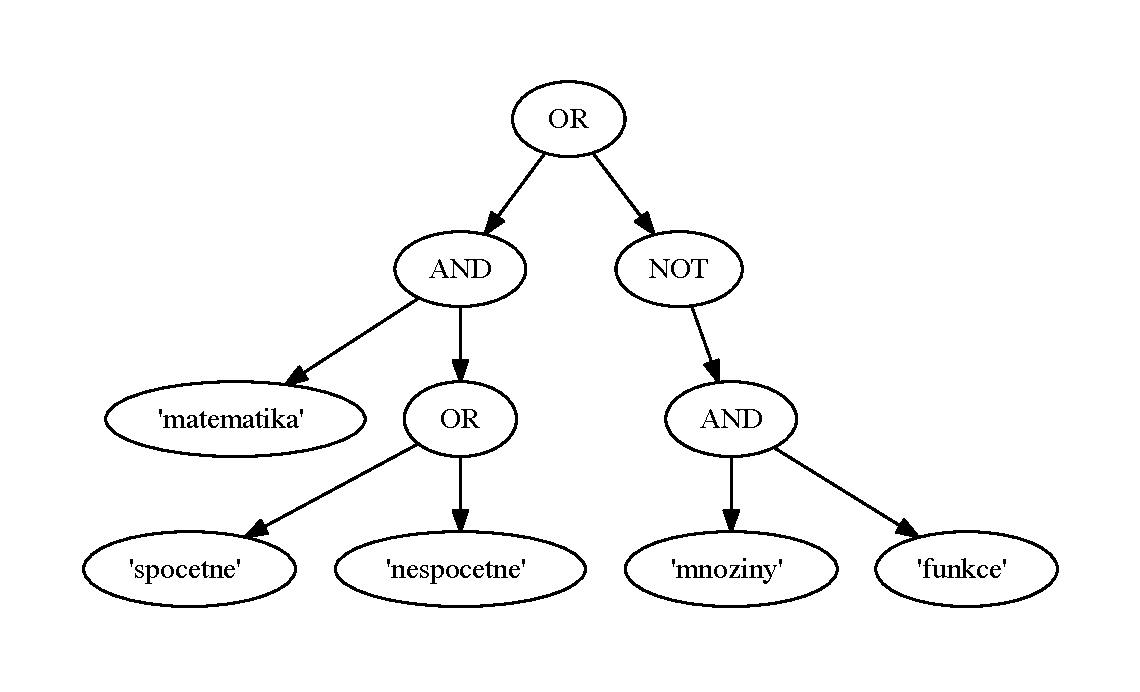
\includegraphics[width=14cm]{obrazky/syntactic_tree.pdf}
  \caption{Syntaktický strom pro dotaz \uv{(matematika AND (spočetné OR nespočetné)) OR (NOT (množiny AND funkce))}}
  \label{fig:syntree}
\end{figure}

Nakonec celý výraz zjednodušíme -- odstraníme uzly, které obsahují stop slova, protože stop slova nepoužíváme při vyhledávání a převedeme slova na stemy. 

\sssection{Vyhledání odpovídajících dokumentů}

Ve chvíli, kdy máme syntaktický strom, se můžeme pustit do dolování dokumentů. K tomu využijeme vybudovaný index, který nám umožňuje snadno zjistit, v jakých dokumentech se vyskytuje dané slovo. Pro účely popisu mechanismu si definujeme funkci $\getdocs$, která bere na vstupu dotaz $Q$ a na výstupu vrací množinu dokumentů, které odpovídají zadanému dotazu. Tato funkce se bude chovat odlišně v závislosti na tom, jak vypadá dotaz $Q$. 

\begin{itemize}
\item Je-li $Q=s$, kde $s$ je nějaké slovo, pak funkce $\getdocs$ vrátí množinu dokumentů, které obsahují dané slovo, což vyčteme z indexu. 
\item Je-li $Q = \alpha \AND \beta$, pak $\getdocs_Q = \getdocs_\alpha \cap \getdocs_\beta$.
\item Je-li $Q = \alpha \OR \beta$, pak $\getdocs_Q = \getdocs_\alpha \cup \getdocs_\beta$.
\item Je-li $Q = \NOT \alpha$, pak $\getdocs_Q = \mathbb{D}\setminus\getdocs_\alpha$, kde $\mathbb{D}$ je množina všech dokumentů.
\end{itemize}

Postupnou aplikací těchto pravidel dostaneme množinu výsledných dokumentů $R$. V dalším kroku tyto dokumenty seřadíme podle relevance. 

\sssection{Seřazení dokumentů}

V současné chvíli máme množinu dokumentů $R$. Aby byl vyhledávač smysluplný, měl by tyto dokumenty seřadit podle toho, jak relevantní dané dokumenty vzhledem k položenému dotazu jsou. To je obecně nelehký úkol. Ve vyhledávači je použit standardní $\tfidf$ algoritmus. 

Abychom mohli ohodnotit jednotlivé dokumenty, potřebujeme znát slova, vůči kterým máme dokumenty ohodnocovat. Odstraníme tak z dotazu všechny operátory a dostaneme množinu všech slov $S$. Vůči těmto slovům budeme dokumenty hodnotit. 

K tomu už využijeme standardní $\tfidf$ algoritmus -- pro každé slovo a pro každý dokument spočítáme jeho $\tfidf$ skóre; poté tato skóre sečteme a dokumenty seřadíme sestupně podle tohoto skóre. Skóre $\score_d$ dokumentu $d$ tak udává vzorec:
$$\score_d=\sum_{s\in S} \tfidf_{s, d}.$$

Nyní seřadíme dokumenty $R$ do $n$-tice $\addh{d_1, d_2, \ldots, d_n}$, kde $n=|R|; d_i\in R \,\forall i$, tak, aby platilo $\score_{d_1} \ge \score_{d_2} \ge \ldots \ge \score_{d_n}$.

Tato seřazená $n$-tice je výstupem algoritmu vyhledávání. 


\newpage
\section{Hledání souvisejících dokumentů}
V této kapitole bude popsána druhá část vyhledávače, která se stará o nalezení souvisejících dotazů. 

\ssection{O co nám půjde}

\sssection{Motivace}

Pokud uživatel položí vyhledávači nějaký dotaz, tak vyhledávač odpoví nějakým seznamem dokumentů, které jsou podle něj nejvíce relevantní. Pokud má uživatel štěstí, bude v tomto seznamu dokument, který zrovna potřebuje najít. Pokud bude mít velké štěstí, pak bude tento dokument na předních místech v seznamu. 

Pokud ale toto štěstí mít nebude a dokument se mu nepodaří nalézt, musí uživatel nějakým způsobem přeformulovat svůj dotaz tak, aby vyhledávač vrátil jinou sadu výsledků. Obecně může upravit dotaz třemi různými způsoby. Může

\begin{enumerate}
\item přidat k dotazu jedno či více slov, díky čehož obrdží méně výsledků,
\item změnit jedno či více slov, díky čehož obdrží podobné výsledky,
\item odebrat jedno či více slov, díky čehož obdrží více výsledků.
\end{enumerate}

V různých situacích se hodí různé postupy. Pokud jsme zadali příliš konkrétní dotaz, bude vhodné odebrat některá klíčová slova dotazu, abychom získali více výsledků. Pokud jsme naopak zadali příliš obecný dotaz, můžeme přidat nějaká klíčová slova, abychom obrželi méně dokumentů, která ale lépe odpovídají na náš dotaz. 

\sssection{Hlavní cíl}

Hlavním cílem vyhledávače je nacházet předchozí úpravy dotazu automaticky. Tyto úpravy můžeme hledat například pomocí historie dotazů, pokud danou historii máme. Pokud uživatel položí dotaz \uv{hosting php}, můžeme se podívat do historie vyhledávání a nalézt všechny dotazy, které obsahují alespoň jedno ze slov v dotazu a z této množiny dotazů pak můžeme nějakým postupem vybrat související dotazy pro všechny tři kategorie úprav. Můžeme například zjistit, že z konkrétnějších dotazů je nejvíce hledaný dotaz \uv{hosting php mysql}, z podobných \uv{server php} a podobně. 

My ale použijeme jiný postup. Všechny související dotazy budeme hledat pouze na základě znalostí sady dokumentů. Nebudeme k tomu využívat žádné dodatečné informace, všechno si spočítáme pouze ze samotných dokumentů.

K tomu využijeme formální konceptuální analýzu dat, která v daných datech vyhledává jisté shluky potenciálně zajímavých dat a zároveň je ukládá do hierarchie, se kterou můžeme dále pracovat. Pro základní představu si můžeme představit výstup FCA jako Hasseův diagram, kde jeden z uzlů představuje aktuální výsledky, které nám vyhledávač zobrazil, \uv{otcové} tohoto uzlu jsou obecnější dotazy, \uv{synové} jsou konkrétnější dotazy a \uv{sourozenci} jsou podobné dotazy. 

\sssection{Výstup vyhledávače}

Jak by měl vypadat výstup vyhledávače? Vyhledávač by měl zobrazit seřazenou sadu klasických výsledků, na tom se nic nemění. Dále by měl spočítat všechny tři kategorie dotazů a pokud nějaké najde, měl by je uživateli zobazit. Tyto návrhy by měl vyhledávač opět seřadit podle relevance, tj. aby první úpravy dotazů byly nejsmysluplnější. Výstup pro dotaz \uv{hosting php} by měl vypadat přibližně takto:

\begin{verbatim}
1. Doc23
2. Doc17
3. ... 

-hosting; -php
~domény hosting; ~databáze php; ~cena hosting
+cena; +databáze; +forum; +formuláře; +kniha
\end{verbatim}

Nejprve máme klasický seznam dokumentů setříděných podle relevance. Následují tři řádky, kde na první místě jsou slova, která můžeme z dotazu dobrat; ta jsou označena symbolem minus. Na dalším řádku jsou dotazy, které můžeme vyhledávat namísto originálního dotazu; jsou označena symbolem tilda. Nakonec jsou slova, která můžeme k dotazu přidat; jsou označena symbolem plus.




%%% Závěr práce v~češtině
\begin{conclusions-cz}
  Závěr práce v češtině.
\end{conclusions-cz}


%%% Závěr práce v~angličtině
\begin{conclusions-en}
  Conclusion in english.
\end{conclusions-en}


\end{document}
